\documentclass[12pt,a4paper]{article} 
\usepackage{graphicx, booktabs, siunitx, amsmath, geometry, float}
\usepackage{subcaption}
\geometry{margin=2.5cm}
\title{M3: Study of Comparators}
\author{Gregorio Jaca (U8L9B9) gregorio.jaca@gmail.com \and Peter Tallosy (K14WR1) peter@tallosy.hu}
\date{\today}

\begin{document}
\maketitle

\begin{abstract}
In this report we show the results obtained from constructing deveral comparator circuits. We investigated a basic operational amplifier comparator, a Schmitt trigger with hysteresis, a relaxation oscillator, and a transistor-based Schmitt trigger. Theoretical calculations for switching thresholds and frequencies were performed and compared against empirical measurements. The results validate the theoretical models and highlight practical aspects of comparator circuit behavior, including the impact of different transistors, like \textmu A741 and TL071 op-amps on performance.
\end{abstract}

\section{Introduction}
In electronics, a comparator is a device that compares two voltages or currents and outputs a digital signal indicating which is larger. It has two analog input terminals and one binary digital output. The output is ideally one of two states, indicating which input is higher. Comparators are fundamental building blocks in analog-to-digital converters, relaxation oscillators, and various sensor-monitoring applications. We implemented comparators using operational amplifiers and transistors.

\section{Theoretical Overview}

\subsection{Basic Comparator}
A basic comparator can be constructed using an operational amplifier (op-amp) without feedback. The op-amp's high open-loop gain causes it to saturate to its positive or negative supply voltage based on the differential input. A more stable configuration uses a voltage divider to set a fixed reference voltage ($U_{ref}$) on one input, against which the other input signal ($U_{in}$) is compared. The switching threshold is determined by this reference voltage.

\subsection{Schmitt Trigger with Hysteresis}
To prevent oscillations at the output when the input signal is noisy or near the threshold, positive feedback is introduced to create hysteresis. This results in two different threshold voltages: an upper threshold ($U_{TH}$) and a lower threshold ($U_{TL}$). The output state depends not only on the input value but also on its previous state. The voltage difference between the two thresholds is the hysteresis width ($U_H = U_{TH} - U_{TL}$).

For the Schmitt trigger, the threshold voltages are given by:
\begin{equation}
    U_{TH} = \frac{R_2}{R_1+R_2}U_{sat+} + \frac{R_1}{R_1+R_2}U_{ref}
\end{equation}
\begin{equation}
    U_{TL} = \frac{R_2}{R_1+R_2}U_{sat-} + \frac{R_1}{R_1+R_2}U_{ref}
\end{equation}
When $U_{ref}$ is ground, and considering the feedback from the output, the thresholds are calculated based on the three resistors and the saturation voltages.

\subsection{Astable Multivibrator}
By modifying the Schmitt trigger circuit, a relaxation oscillator (astable multivibrator) can be created. This circuit generates a continuous square wave without any input signal. The op-amp charges and discharges a capacitor ($C$) through a resistor ($R$) between the two threshold voltages of the Schmitt trigger. The frequency of oscillation is determined by the RC time constant and the resistor values of the voltage divider. The period ($T$) is given by:
\begin{equation}
    T = 2 \cdot R_1 \cdot C \cdot \ln\left(\frac{U_{sat+} - U_{TL}}{U_{sat+} - U_{TH}}\right)
\end{equation}

\subsection{Transistor Schmitt Trigger}
A Schmitt trigger can also be implemented using discrete transistors. The positive feedback is achieved by coupling the collector of the second transistor to the base of the first. The circuit has two stable states, with one transistor in saturation and the other in cutoff. The switching thresholds are determined by the resistor values and the transistor characteristics.

\section{Experimental Work and Results}

\subsection{M1: Basic Comparator}
A comparator circuit was built using a \textmu A741 op-amp. The reference voltage was set by a voltage divider with $R_1 = \SI{22}{\kilo\ohm}$ and $R_2 = \SI{10}{\kilo\ohm}$, and a supply voltage of $\pm\SI{5}{V}$.

\textbf{Theoretical Threshold:}
The theoretical threshold voltage is calculated using the voltage divider formula:
\begin{equation}
U_{threshold,calc} = U_{supply+} \times \frac{R_2}{R_1 + R_2} = \SI{5}{V} \times \frac{\SI{10}{\kilo\ohm}}{\SI{22}{\kilo\ohm} + \SI{10}{\kilo\ohm}} = \SI{1.56}{V}
\end{equation}

\textbf{Measurements:}
The input voltage $U_2$ was varied, and the switching point was found to be $1.5 \pm 0.1~\text{V}$ , which is, up to the measurement error, within the expected range. We also measured the other voltages:
\begin{itemize}
    \item $U_1 = \SI{1.575}{V}$ (constant).
    \item For $U_2 < \SI{1.5}{V}$, the output was $U_{out} = \SI{4.47}{V}$.
    \item For $U_2 > \SI{1.5}{V}$, the output was $U_{out} = \SI{-3.14}{V}$.
\end{itemize}
The measured threshold is in close agreement with the calculated value. The output voltages represent the saturation levels of the op-amp and depended on the power supply.

\subsection{M2: Schmitt Trigger}
The previous circuit was modified by adding a positive feedback resistor $R_3 = \SI{99.5}{\kilo\ohm}$ (nominally $\SI{100}{\kilo\ohm}$) to create a Schmitt trigger.



\begin{figure}[H]
    \centering
    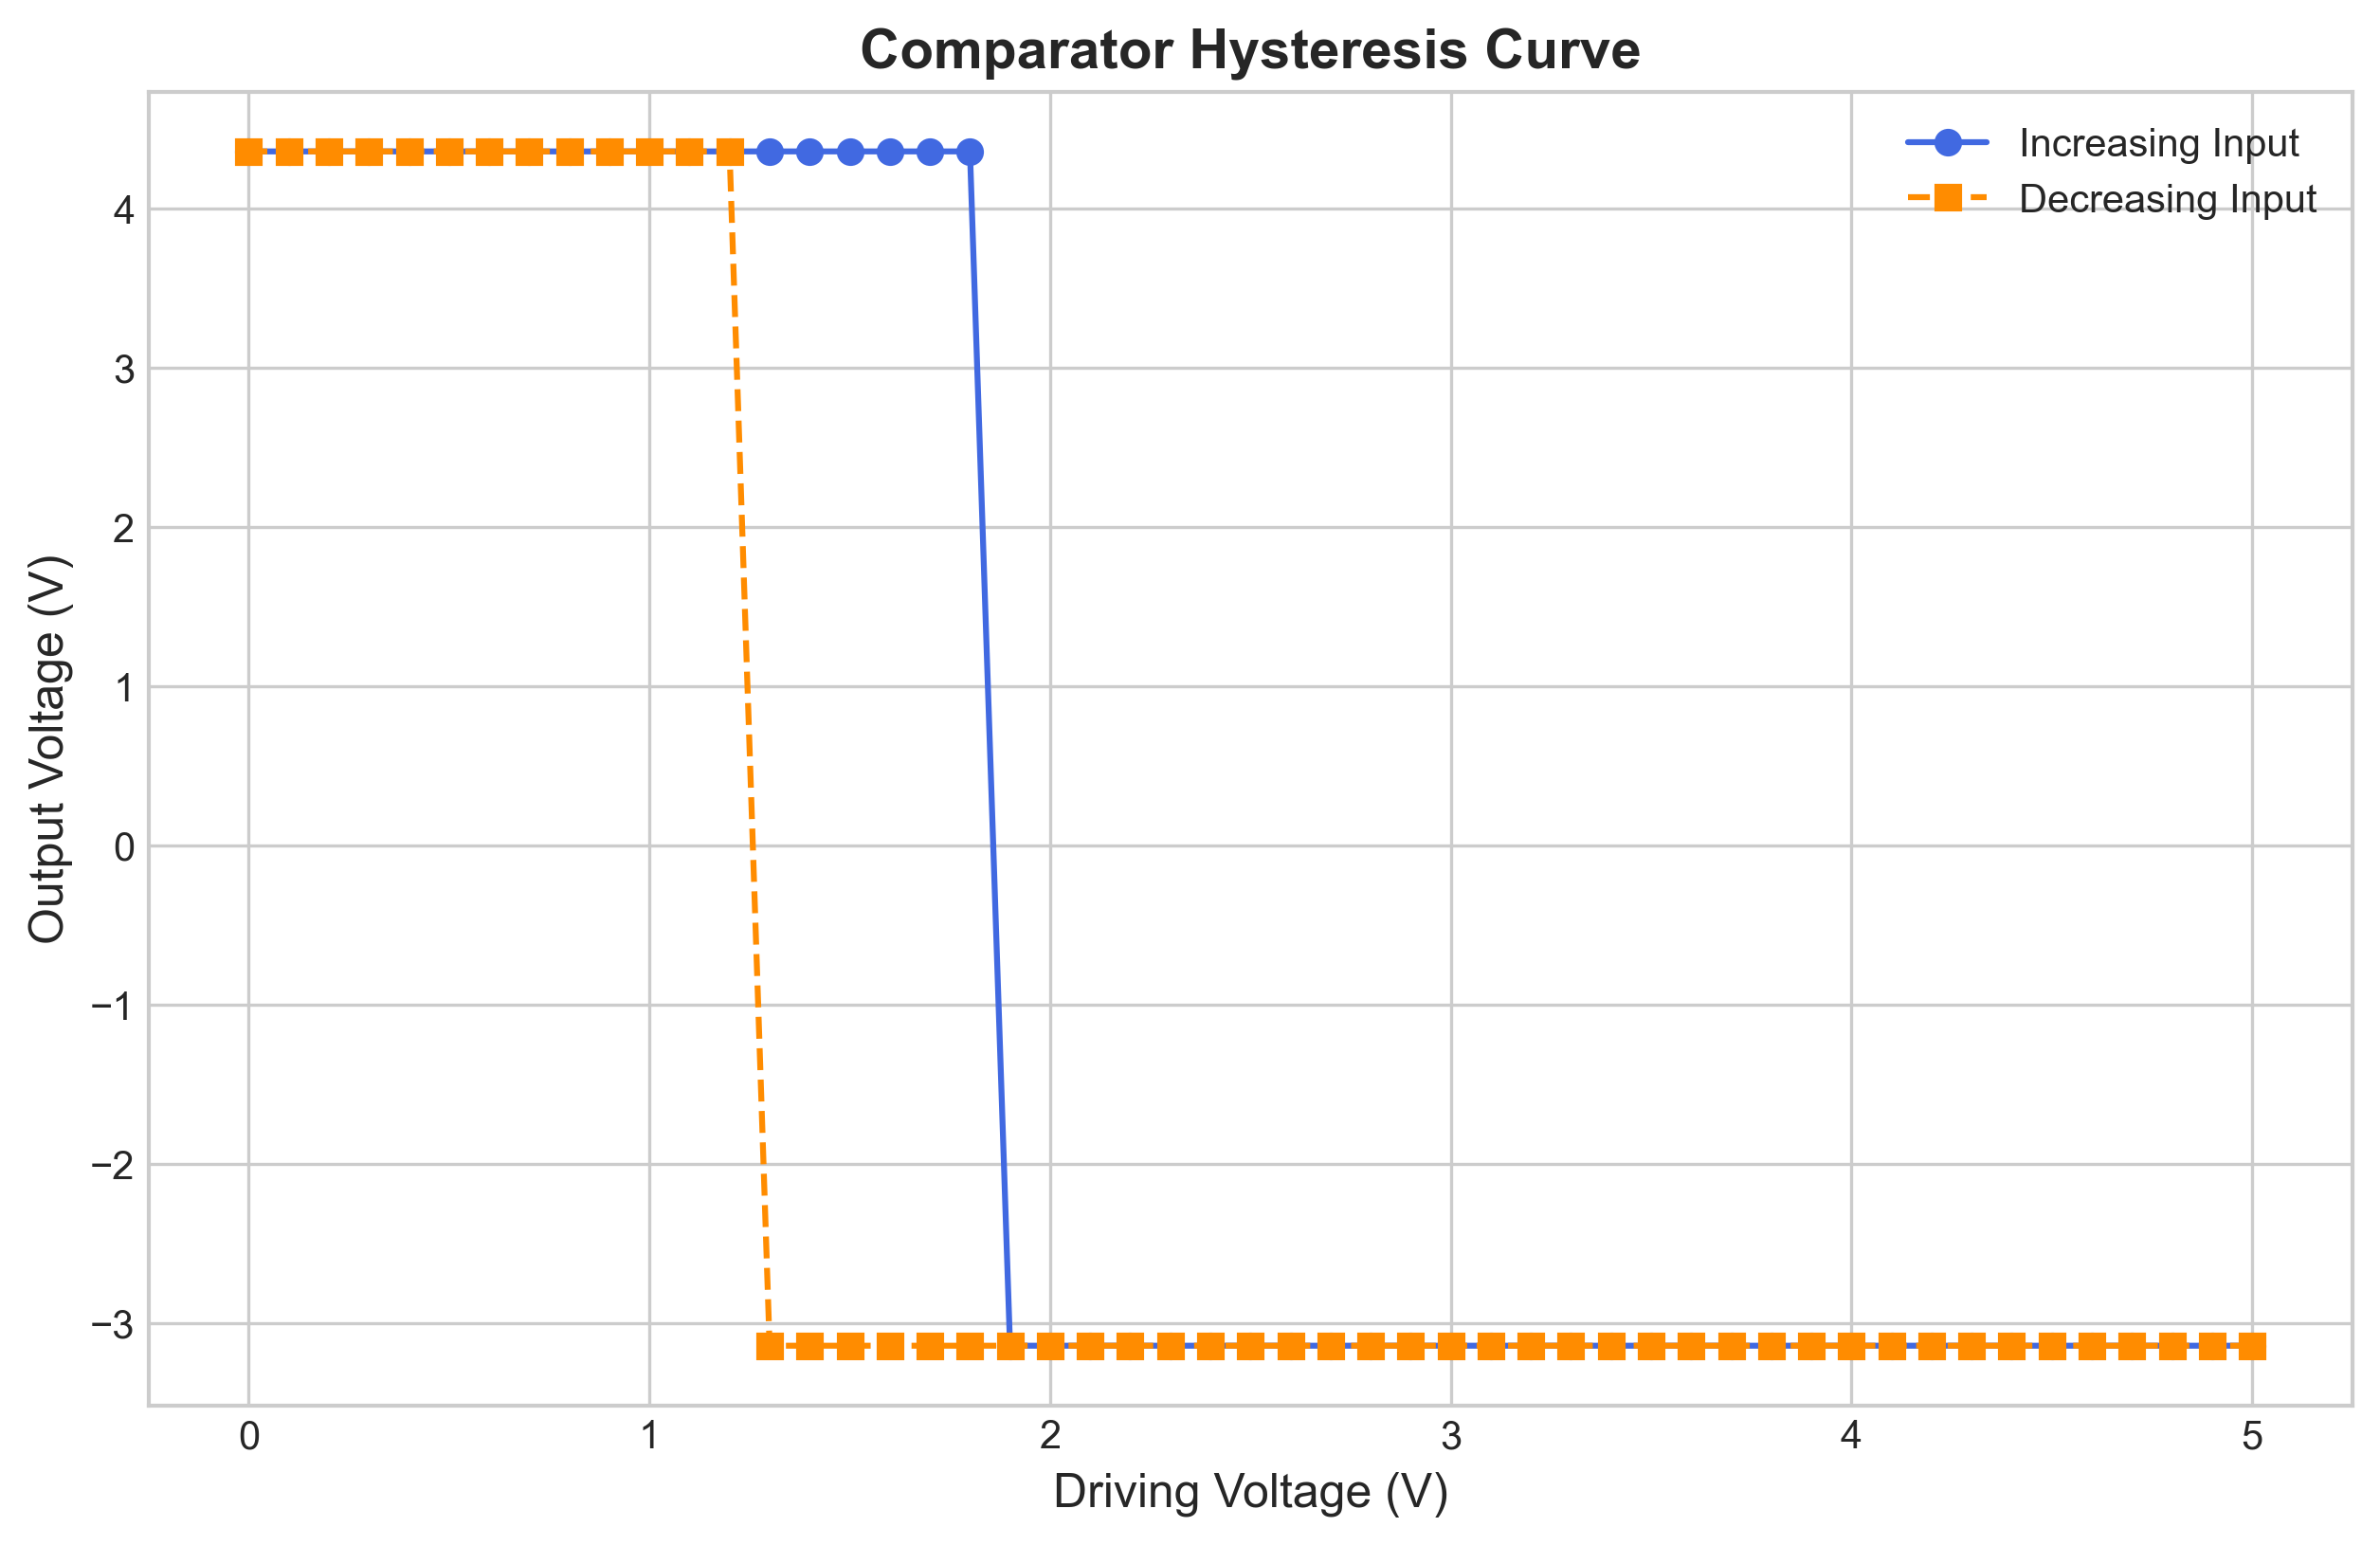
\includegraphics[width=0.6\linewidth]{plot2.png}
    \caption{.}
    \label{fig:plot2}
\end{figure}

\textbf{Measurements:}
\begin{itemize}
    \item Upper threshold (increasing $U_2$): $U_{TH,meas} = \SI{1.85}{V}$. $U_1 = \SI{1.754}{V}$ 
    \item Lower threshold (decreasing $U_2$): $U_{TL,meas} = \SI{1.25}{V}$. $U_1 = \SI{1.273}{V}$
    \item Hysteresis width: $U_H = U_{TH,meas} - U_{TL,meas} = \SI{1.85}{V} - \SI{1.25}{V} = \SI{0.6}{V}$.
    \item Output voltages remained consistent: $U_{out,high} = \SI{4.36}{V}$ and $U_{out,low} = \SI{-3.14}{V}$.
\end{itemize}
The measured thresholds are close to the theoretical values, and the circuit exhibits clear hysteresis. This is benefitial in cases of noisy signal or being close to the threshold voltage, where (if there were no hysteresis) small amounts of noise could change the comparator output. Hysteresis makes it more robust. The values for $U_1$ remained constant within each region, but if we increases the input voltage above $\SI{5}{V}$, then $U_1$ increases with it.

\subsection{M3: Relaxation Oscillator}
An astable multivibrator was constructed using a TL071 op-amp with $R_1 = \SI{10}{\kilo\ohm}$, $R_2 = \SI{10}{\kilo\ohm}$, and $R_3 = \SI{22}{\kilo\ohm}$. The goal was to achieve an oscillation frequency of $f = \SI{12}{kHz}$.

\textbf{Capacitance Calculation:}
The required capacitance $C$ was calculated to be approximately $\SI{6.92}{nF}$. A standard capacitor of $C = \SI{6.8}{nF}$ was chosen.
With this capacitor, the expected frequency is:
\begin{equation}
f_{exp} = \frac{1}{2 \cdot C \cdot R_1 \cdot \ln(\frac{U_{sat+} - U_{TL}}{U_{sat+} - U_{TH}})} \approx \SI{12.21}{kHz}
\end{equation}

We observed the waveform at the oscilloscope and found a frequency of $\SI{10.9}{kHz}$, which is close but smaller than expected. We suspect that some added capacitance introduced by the op-amp, reducing the frequency of oscillation.

\begin{figure}[H]
    \centering
    \begin{subfigure}[b]{0.48\linewidth}
        \centering
        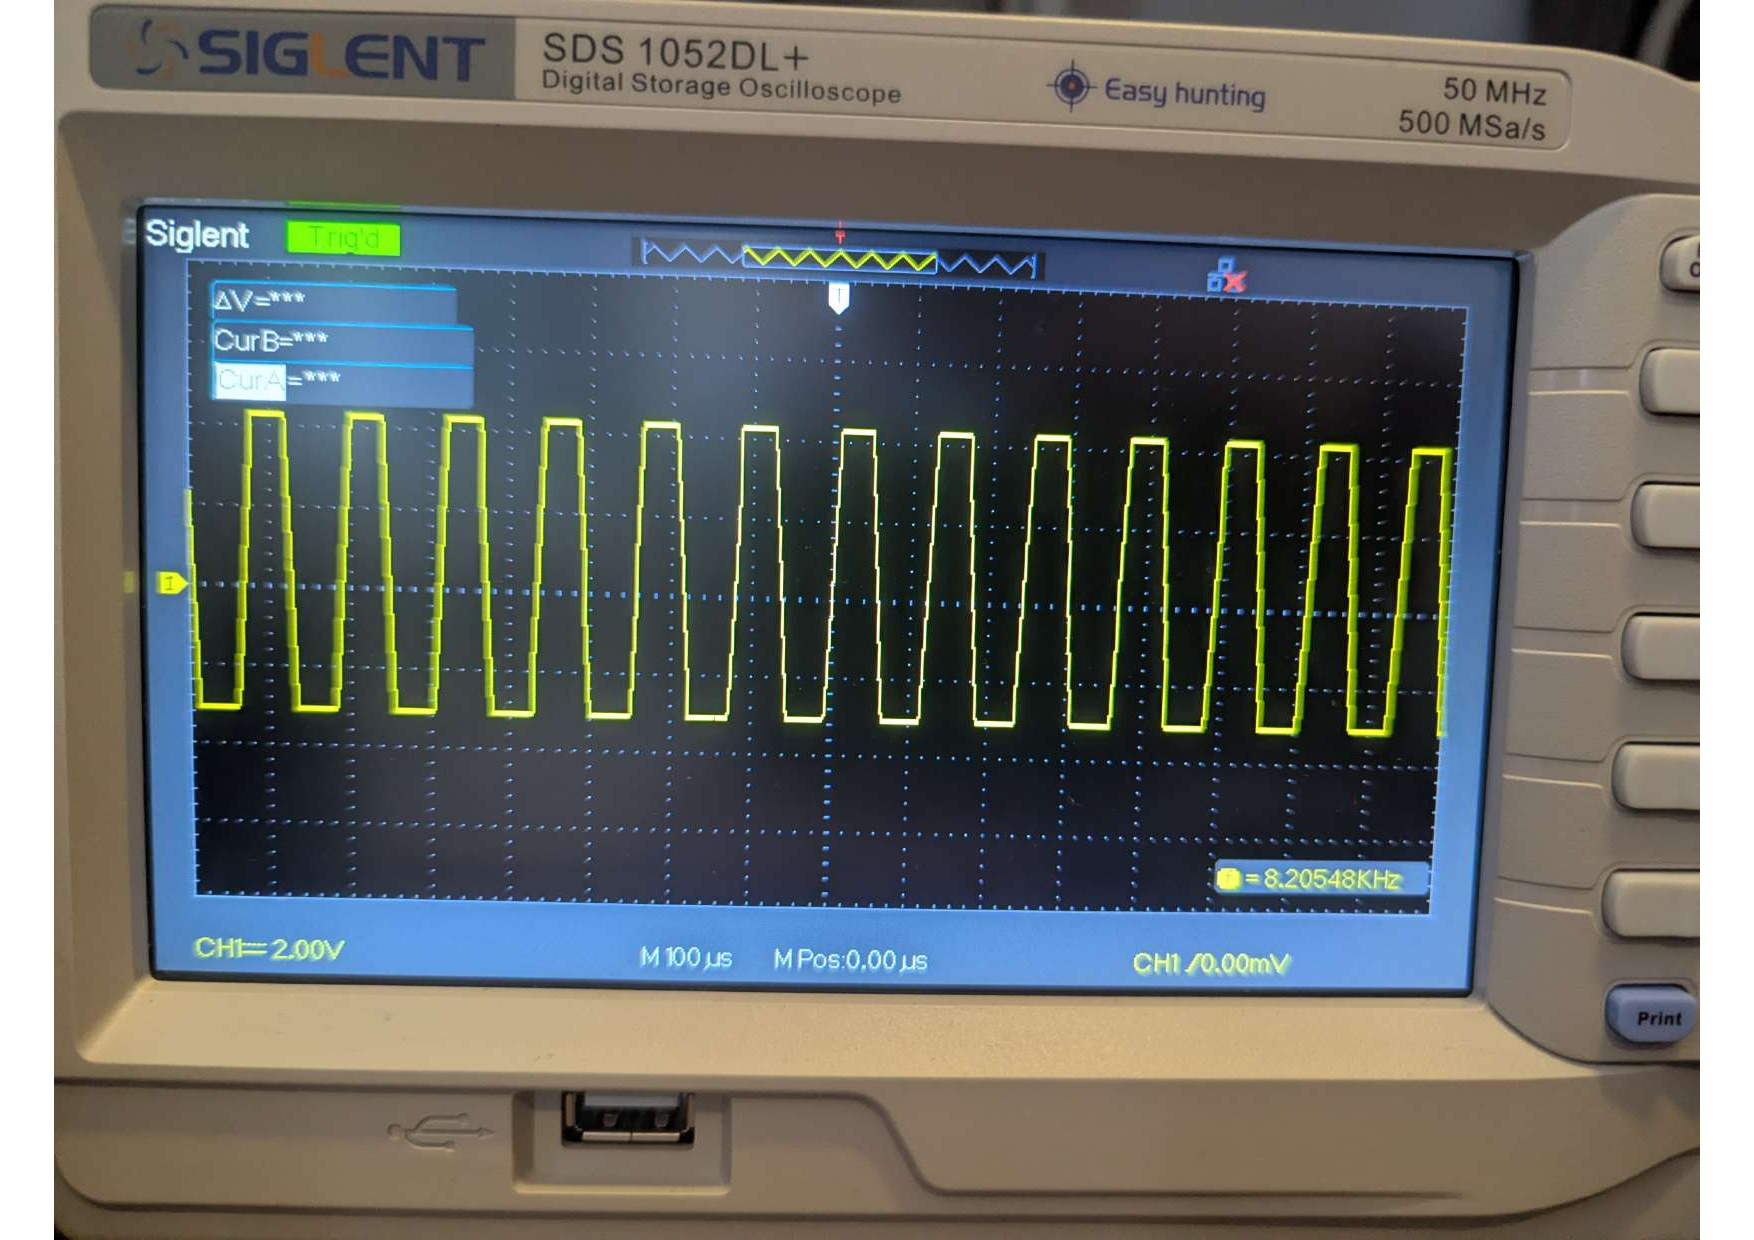
\includegraphics[width=\linewidth]{ua741.pdf}
        \caption{\textmu A741 op-amp waveform}
    \end{subfigure}\hfill
    \begin{subfigure}[b]{0.48\linewidth}
        \centering
        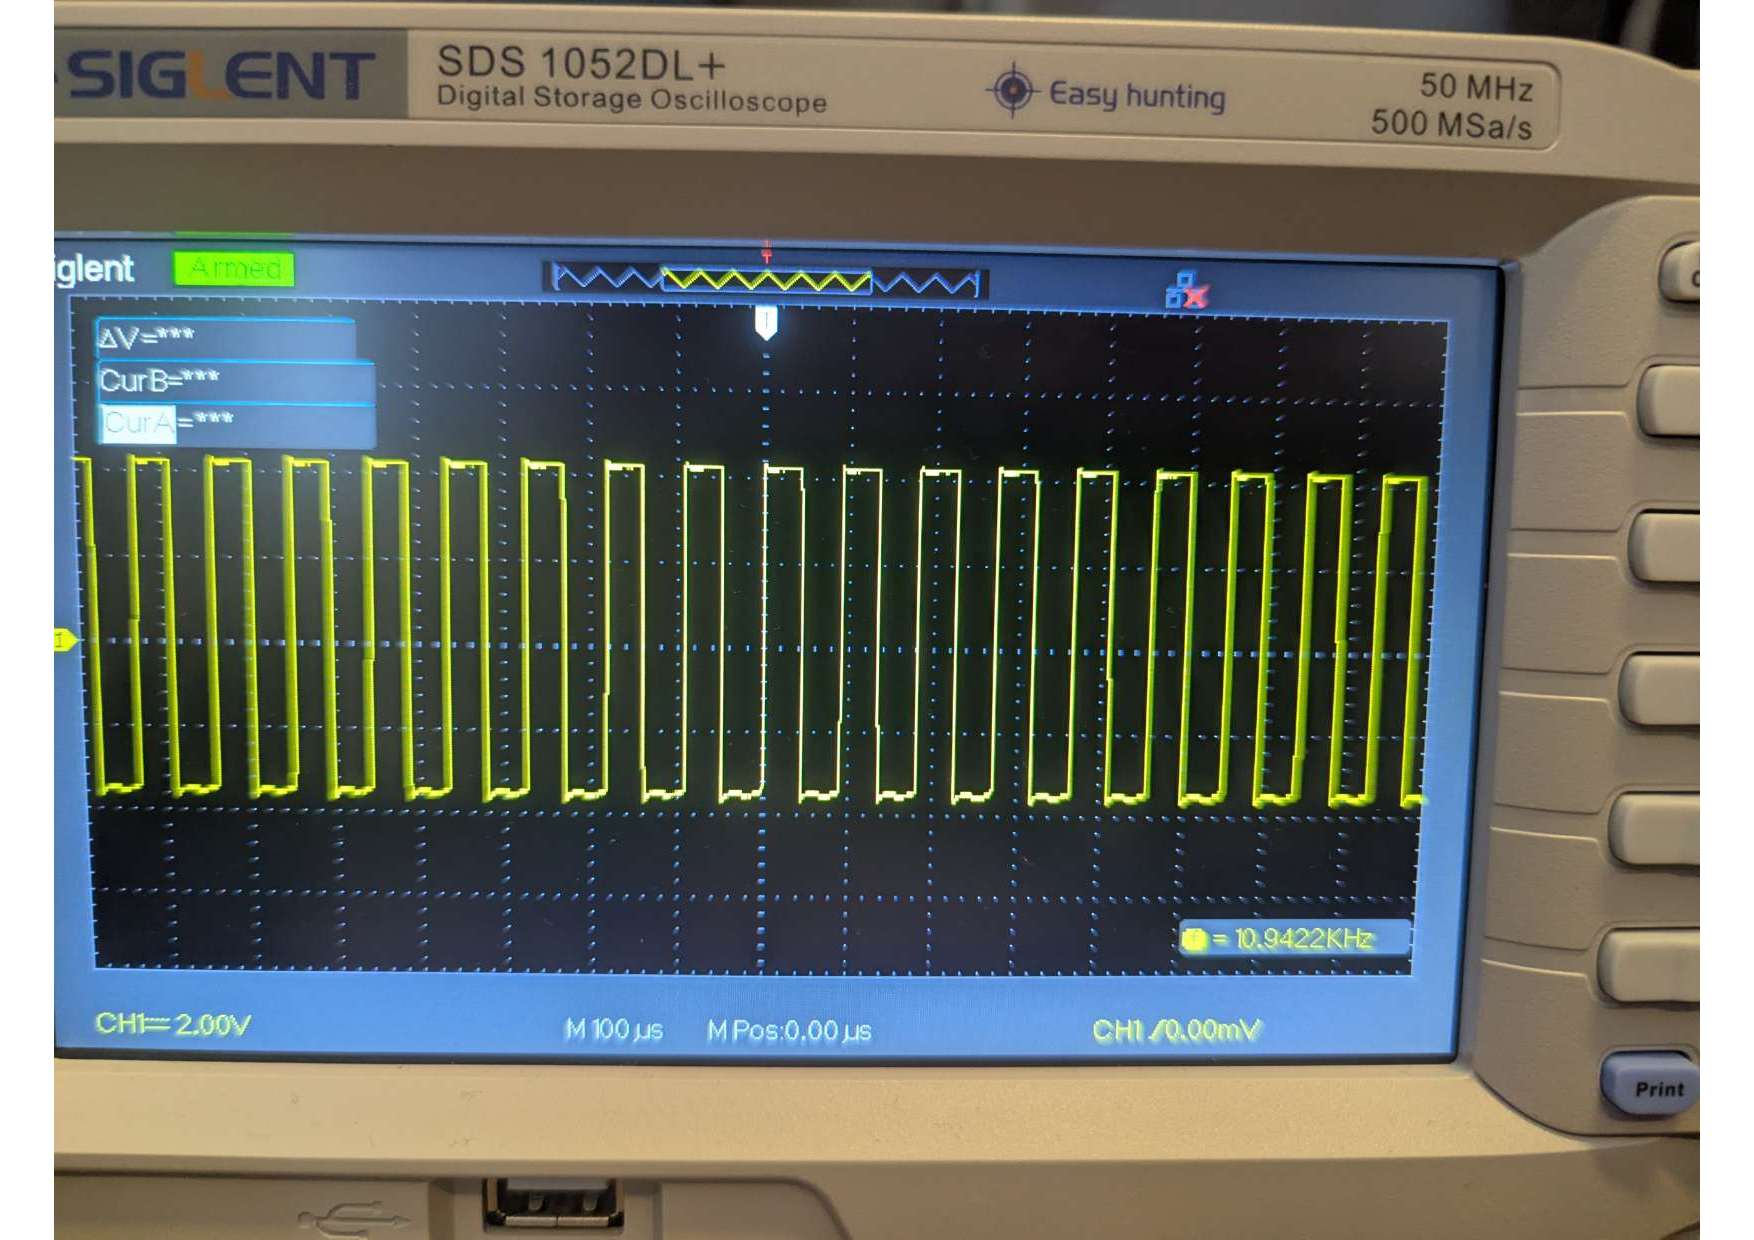
\includegraphics[width=\linewidth]{tl071.pdf}
        \caption{TL071 op-amp waveform}
    \end{subfigure}

    \label{fig:waveforms}
\end{figure}

The TL071 was replaced with a \textmu A741 op-amp and the procedure repeated. The measured frequency was $\SI{8.2}{kHz}$.
This represents a significant decrease of 32.87\% from the expected frequency. This deviation is lead us to believe to the internal characteristics of the \textmu A741, such as a higher internal stray capacitances, which effectively increase the total capacitance in the timing circuit, thus lowering the oscillation frequency. In order to validate this we looked at datasheets for these transistors. The TL071 has an internal compensation capacitance of around 18 pF, while \textmu A741 has a capacitance of 1.4 pF. This is contrary to what we were expecting. This lead us to believe that it was the effect of the slew rate. The TL071 has an slew rate of around 13 V / \textmu s, while \textmu A741 has a slew rate of 0.5 V/ \textmu s. This explains that \textmu A741 has a smaller frequency. This shows the effect of different electronic components in a circuit like this.

\subsection{M4: Transistor Schmitt Trigger}
A Schmitt trigger was built using two BC182 transistors.

\textbf{Theoretical Thresholds:}
The theoretical thresholds depend on the saturation voltages of the transistors and the resistor network. Initial calculations suggested thresholds around $\SI{0.6}{V}$.

\begin{itemize}
    \item Increasing input $U_{in}$: At \SI{0.95}{V}, the output switched. 
    \item Decreasing input $U_{in}$: At $\SI{0.65}{V}$, the output switched back. 
    \item High value $U_{high} = \SI{5.01}{V}$
    \item Low valie  $U_{low} = \SI{0.45}{V}$.
    \item Hysteresis width: $U_H = \SI{0.95}{V} - \SI{0.65}{V} = \SI{0.3}{V}$.
\end{itemize}

\begin{figure}[H]
    \centering
    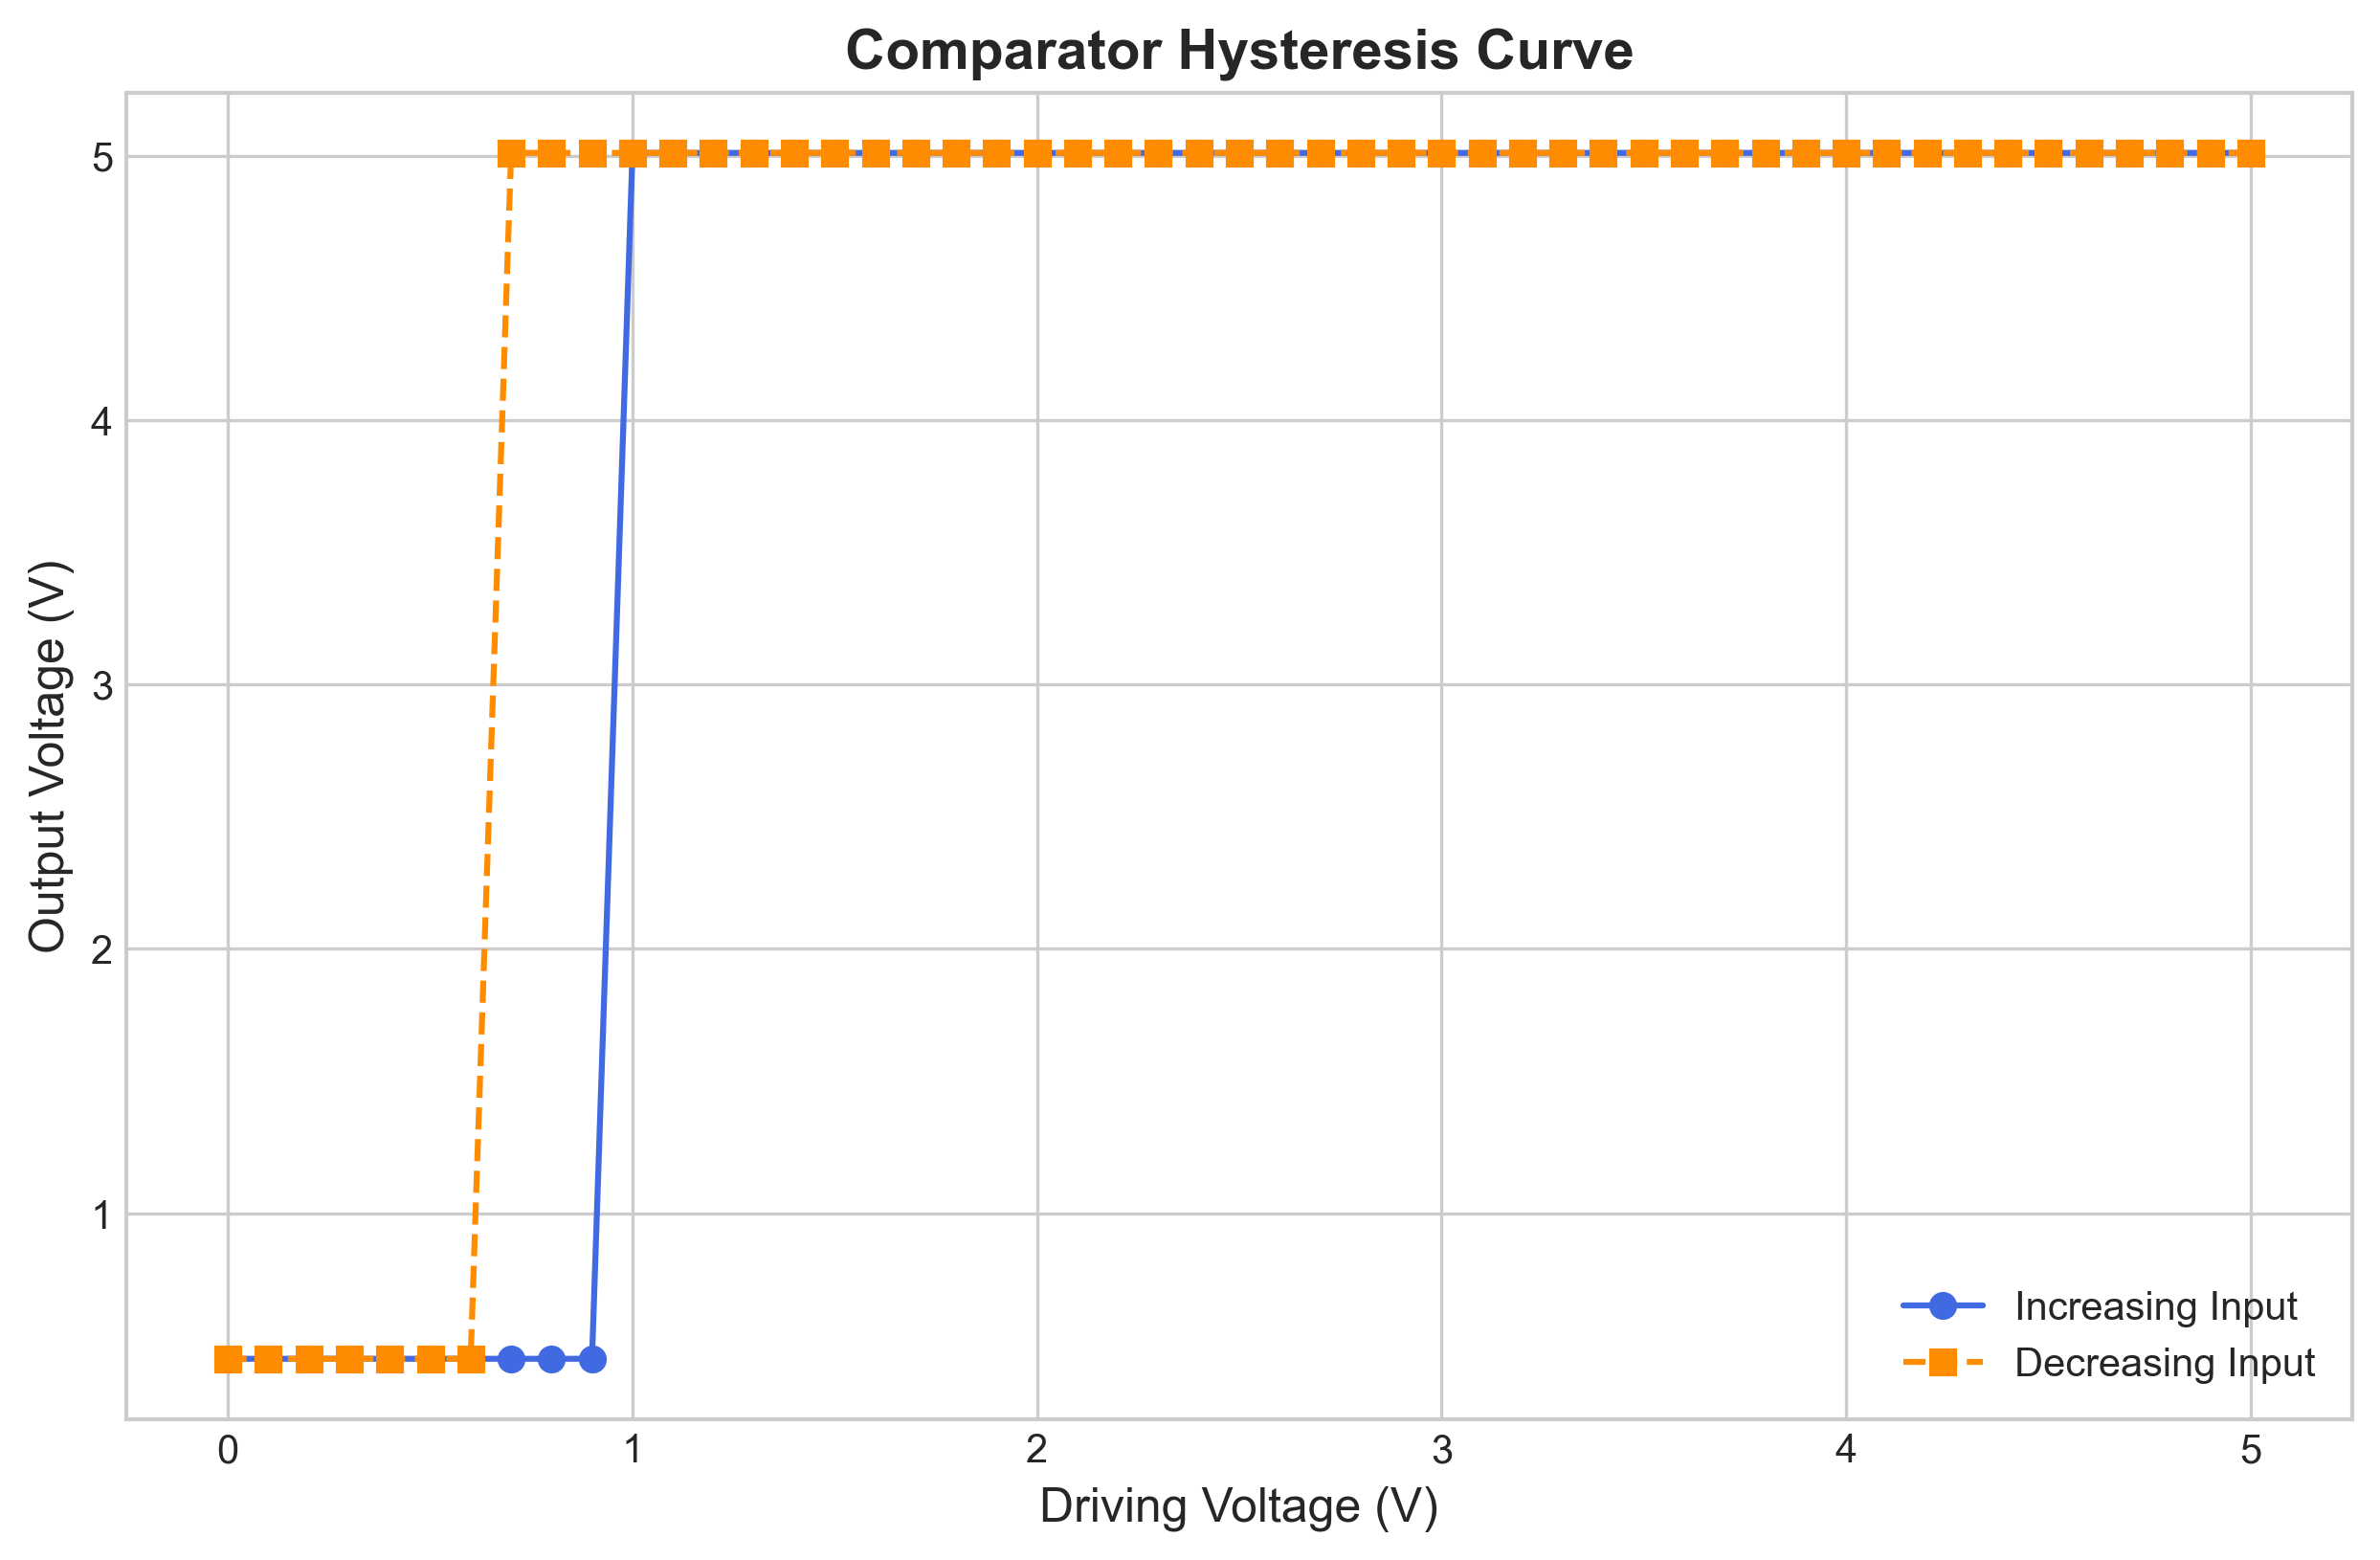
\includegraphics[width=0.7\linewidth]{plot4.png}
    \caption{Hysteresis can be observed.}
    \label{fig:excel_plot}
\end{figure}

The circuit functioned as expected, demonstrating the principle of a transistor-based Schmitt trigger. The circuit can switch with either one or the other transistor conducting. Hysteresis is caused by the different resistance values at the collector of the two transistors.



\section{Equipment Used}
\begin{itemize}
    \item Op-Amps: \textmu A741, TL071
    \item Transistors: BC182
    \item DC Power Supply: Siglent SPD3303C
    \item Digital Multimeter: Siglent SDM 3045X and UNI-T UT334+
    % \item Function Generator: RIGOL DG811 SiFi II 20MHz AWG
    \item Oscilloscope: SIGLENT SDS 1072CML Digital Oscilloscope
    \item Resistors and Capacitors of various values. Breadboard and Wires.
\end{itemize}

\section{Conclusion}

In this laboratory excercise we could build and measure the required circuits, understanding their operation and behavior. We observed that the measured switching thresholds in the basic comparator and Schmitt trigger circuits closely matched the theoretical predictions. The astable multivibrator experiment highlighted the significant impact of op-amp choice on circuit performance, with the TL071 performing closer to the ideal model than the older \textmu A741, primarily due to differences in slew rate. The transistor-based Schmitt trigger also performed as expected, confirming that discrete components can be used to achieve the same functionality. Overall, the experiments provided understanding into the design and behavior of comparators, which are used in analogue-digital convertors and circuits.

\end{document}
